\documentclass[12pt,twocolumn,tighten]{aastex62}
%\pdfoutput=1 %for arXiv submission
\usepackage{amsmath,amstext,amssymb}
\usepackage[T1]{fontenc}
\usepackage{apjfonts}
\usepackage[figure,figure*]{hypcap}
\usepackage{graphics,graphicx}
\usepackage{hyperref}
\usepackage{comment}

\renewcommand*{\sectionautorefname}{Section} %for \autoref
\renewcommand*{\subsectionautorefname}{Section} %for \autoref

%% Reintroduced the \received and \accepted commands from AASTeX v5.2.
%% Add "Submitted to " argument.
%\received{---}
%\revised{---}
%\accepted{---}
%\submitjournal{}

\shortauthors{Bouma et al.}
\shorttitle{Vetting Report Description Document}

%%%%%%%%%%%%%%%%%%%%%%%%%%%%%%%%%%%%%%%%%%
% BEGIN CUSTOM SHORT-CUT COMMANDS

\newcommand{\stscilink}{\url{archive.stsci.edu/prepds/cdips}}
\newcommand{\stscivetlink}{\url{archive.stsci.edu/prepds/cdips/vetting}}

% END CUSTOM SHORT-CUT COMMANDS
%%%%%%%%%%%%%%%%%%%%%%%%%%%%%%%%%%%%%%%%%%

%%%%%

%\NewPageAfterKeywords

\begin{document}

\title{
  Cluster Difference Imaging Photometric Survey.
  Vetting Report Description Document
}

\correspondingauthor{L. G. Bouma}
\email{luke@astro.princeton.edu}

\author[0000-0002-0514-5538]{L. G. Bouma}
\affiliation{ Department of Astrophysical Sciences, Princeton
University, 4 Ivy Lane, Princeton, NJ 08540, USA}
%
\author[0000-0001-8732-6166]{J. D. Hartman}
\affiliation{ Department of Astrophysical Sciences, Princeton
University, 4 Ivy Lane, Princeton, NJ 08540, USA}
%
\author[0000-0002-0628-0088]{W. Bhatti}
\affiliation{ Department of Astrophysical Sciences, Princeton
    University, 4 Ivy Lane, Princeton, NJ 08540, USA}
%
\author[0000-0002-4265-047X]{J. N. Winn}
\affiliation{ Department of Astrophysical Sciences, Princeton
University, 4 Ivy Lane, Princeton, NJ 08540, USA}
%
\author[0000-0001-7204-6727]{G. \'A. Bakos}
\affiliation{ Department of Astrophysical Sciences, Princeton
University, 4 Ivy Lane, Princeton, NJ 08540, USA}

\begin{abstract}
To find planet candidates in clusters, we make vetting reports using
our light-curves \citep{bouma_cdips_2019} and auxiliary data.  This
document describes the CDIPS planet candidate vetting reports
uploaded by \texttt{bouma} to ExoFOP-TESS 2020-01-20 through
2020-05-01.  Earlier versions of this document are available at
\url{lgbouma.com/notes}.
\\

\end{abstract}

%\keywords{
%	Transit photometry (1709),
%	Stellar ages (1581)
%}

%%%%%%%%%%%%%%%%%%%%%%%%%%%%%%%%%%%%%%%%%%
\section{Vetting Report Description}
\label{appendix:vetreport}

The NASA team and MIT teams \citep{jenkins_spoc_2010,huang_tess_2018}
produce vetting reports to assess the quality of planet candidates
identified through their transiting planet serach pipelines.

One goal of the CDIPS project is to detect transiting planets with
known ages.  Therefore our vetting reports include information to help
assess {\it (a)} whether the transiting planet candidate is real, and
{\it (b)} whether the reported age is correct.
The code used to make these reports is available online\footnote{
  \url{https://github.com/lgbouma/cdips/tree/57274b}}.

Figures~\ref{fig:pg1} to~\ref{fig:pg7} summarize the document
construed for these purposes.  The planet candidate chosen for these
figures (Gaia-DR2 \texttt{3050033749239975552} = TIC
\texttt{125192758}) was chosen because it showcases many of the
vetting report features, in this case for a neighboring eclipsing binary.

\subsection{Transit search summary}
\label{sec:pg1}

Figure~\ref{fig:pg1}.  Periodograms from TLS and phase-dispersion
minimization, calculated with \texttt{astrobase.periodbase}, are shown
in the top left and top center
\citep{bhatti_astrobase_2018,hippke_TLS_2019,stellingwerf_period_1978}.
The top three peaks from each method are shown in the second and third
rows; the raw light-curve is in the top-right. A finder chart
is inset to the top left, with the 1.5-pixel radius aperture
used to extract the light-curve in orange.
The finder charts are from The Second Digitized Sky Survey (Red); they
are pulled from NASA's \texttt{skyview} service\footnote{See
\url{https://skyview.gsfc.nasa.gov/current/cgi/survey.pl} and
\url{http://archive.stsci.edu/dss/acknowledging.html}}.

\subsection{Light-curve diagnostics}
\label{sec:pg2}

Figure~\ref{fig:pg2}.
Time-series of raw flux (\texttt{IRM2}),  TFA-detrended flux
(\texttt{TF2}), stellar-variability ``detrended flux'', and the background
are shown as a function of barycentric Julian date.  The overplotted
dashed vertical lines are the ephemeris of the highest-power TLS peak
from Figure~\ref{fig:pg1}.  An important visual check is whether the flux
dips are correlated with changes in the background level -- in this
case, they are not.  The standard deviation and TESS magnitude are
quoted in the upper right.  The red line in the top
plot is a spline fit, which in this case helped in
finding the eclipse signal.

The spline is an optional feature: it is only fitted and removed if
the star is found to be ``variable'' (the Lomb-Scargle peak period is
found with false alarm probability below $10^{-5}$, within the TFA light-curves). The spline is a
robust penalized B-spline, which is a B-spline with knot-length
automatically determined via cross-validation
\citep{eilers_flexible_1996}. The idea behind the cross-validation is
that more knots leads to smaller residuals on training data, but
larger errors when tested on the entire dataset.  We used the
\texttt{wotan} implementation\footnote{
We use \texttt{wotan} versions greater than \texttt{1.4}. Before \texttt{2020-03-01}, an earlier version
was used, which led to qualitatively worse detrending performance for a subset
of light-curves due to a floating point truncation error. See \texttt{\url{https://github.com/hippke/wotan/issues/51}}.
}, which is a wrapper to the
\texttt{pyGAM} spline fitter, with $2\sigma$ clipping of outliers from
the fit residuals at each iteration
\citep{serven_pygam_2018_1476122,hippke_wotan_2019}.  The maximum
number of spline knots was set to 50, which for each TESS sector
($\approx 25\,{\rm days}$) is commensurate with a $\approx0.5\,{\rm
day}$ window.

Whenever the TFA light-curve is found to be variable, the ``stellar variability detrended flux'' is
the result of dividing the raw \texttt{IRM2} flux by the best-fit spline\footnote{
Before \texttt{2020-03-01}, this definition was different. For the initial
single-sector processing of S6-S11, it was the result of dividing the \texttt{TFA2} flux
by the best-fit spline.
}.
This is the light-curve that is then searched for transiting planets, and used
in {\it e.g.}, Figure~\ref{fig:pg1} and Figure~\ref{fig:pg3}.
If the TFA light-curve is not found to be variable, then the \texttt{TFA2} light-curve is used for
this purpose.


\subsection{Transit diagnostics}
\label{sec:pg3}

Figure~\ref{fig:pg3}.
The plots show the maximally-detrended light-curve (top); the
phase-folded light-curve centered over $\pm3$ transit durations of the
primary transit (middle left); the secondary eclipse (middle right);
the odd-numbered transits (lower left); and the even-numbered transits
(lower right).
Also shown is the best-fit TLS template model --- by default, this
assumes a non-grazing geometry (see \citealt{hippke_TLS_2019}).

The stellar parameters ($T_{\rm eff}, R_\star, M_\star$) are taken
from TICv8 when available \citep{stassun_TIC8_2019}.  For the stellar
radius, if TICv8 does not quote a radius, neither will the vetting
report.  If TICv8 gives a stellar radius, but does not give
a stellar mass, we interpolate the mass using the radius and the 
\citet{pecaut_intrinsic_2013}
table, under the assumption that the star is a dwarf.
%\footnote{\url{http://www.pas.rochester.edu/~emamajek/EEM_dwarf_UBVIJHK_colors_Teff.txt}}.
The effective temperatures calculated by TICv8 were estimated from an empirical
color relation involving Gaia $G_{\rm Bp}$ and $G_{\rm Rp}$ magnitudes.  These
observed colors were dereddened first, using Pan-STARRS dust maps
\citep{green_galactic_2018} for declinations above $-30^\circ$, and the
\citet{schlegel_maps_1998} maps otherwise.

The first eight lines of text are parameters determined from the
best-fitting TLS model.  The one exception is the planet radius, which
uses the stellar radius as noted above.  The ``flux contamination''
(\texttt{TICCONT}) from neighboring stars is {\it never} taken into
account, because transit depth dilution does not affect image
subtraction analyses in the same manner as aperture-photometry
reductions.  The significance of the odd-to-even asymmetry is quoted,
but given the strong rotational variability in this object
(Figure~\ref{fig:pg2}), the apparent odd-even asymmetry could have
been caused by the detrending process.  To estimate the transit to
occulation depth ratio $\delta_{\rm tra}/\delta_{\rm occ}$, the
phase-folded light-curve is also fit by a sum of two gaussians (in
this case, the fit failed).  ``AstExc'' refers to the Gaia-DR2
astrometric excess, which can indicate hints of astrometric binarity
in the system.  ``$d_{\rm geom}$'' is the geometric distance from
\citet{bailer-jones_distances_2018}.  ``$R_\star + M_\star \rightarrow
T_{b0}$'' gives the duration of a zero-eccentricity central transit
based on the TICv8 stellar radius and masses discussed above.

\subsection{Light-curves for increasing aperture sizes}
\label{sec:pg4}

Figure~\ref{fig:pg4}.
Apertures of radius 1, 1.5, and 2.25 pixels are shown in maximally detrended
light-curves from top to
bottom.  The blue line is the reference transit depth from the
best-fitting TLS model.  Changes in depth with increasing aperture
size can indicate that the source of variability is off-center from
the aperture, suggesting a photometric blend.

\subsection{Cluster membership assessment diagnostics}
\label{sec:pg5}

Figure~\ref{fig:pg5}.
The star was considered a candidate cluster member by the source(s)
listed under ``Reference'', in this case
\citet{cantat-gaudin_gaia_2018}.  The name used in their catalog was
in this case a Gaia-DR2 identifier, which can be
back-referenced to find the membership probability they assigned this
star for being in NGC 2323.  The base catalog however for this page
of plots is \citet{Kharchenko_et_al_2013}, due to its homogeneous
parameter determination procedure (particularly for age).  If a match to
the \citet{Kharchenko_et_al_2013} catalog is found, then the subplots on
this page are populated; otherwise, they are not.  Top-left shows the
parallax, with orange points sampled from the Gaia-DR2 posterior, black
points the other cluster members in the {\it Kharchenko catalog} (not
the catalog claiming membership), and the blue line the claimed
Kharchenko parallax for the cluster.  A number of field contaminants in
the Kharchenko catalog are visible in this case.  Top-right are the Gaia
proper motions, where against black points are cluster members from
Kharchenko, and the orange is the target star.  Bottom-left is the
color-magnitude diagram, and bottom-right are the on-sky positions.  In
the text, \texttt{N1sr2} is the number of $1\sigma$ cluster members
reported by \citet{Kharchenko_et_al_2013} within the cluster angular
radius; $\log t$ is the base-10 logarithm of the age in years;
\texttt{type} matches the type codes provided by
\citet{Kharchenko_et_al_2013}; ``\texttt{Note}'' gives the description
of the cluster from \citet{Kharchenko_et_al_2013}, if any is available.
Extra caution must be taken when interpreting this set of plots, since
they can only show disagreement between the observed star's properties
and those of the listed Kharchenko members (and the latter is in some cases
incomplete or otherwise biased).

\subsection{Imaging variability diagnostics}
\label{sec:pg6}

Figure~\ref{fig:pg6}.
This page helps diagnose which stars are producing the observed
variability.  Top-left and top-center are the mean out-of-transit
(OOT) and mean in-transit calibrated images (created separately from our
image-subtraction analysis, using \texttt{TESScut},
\citealt{brasseur_astrocut_2019}).  The OOT images are based on the same
number of exposures as the in-transit images and split evenly before
and after each transit
\citep[following][]{bryson_identification_2013,kostov_l9859_2019}.
The yellow star is the target's position from TICv8; 
small red crosses are WCS-projected locations of neighbor stars.

Middle-left is the most important sub-panel: the difference between
the OOT and in-transit mean images.
If the variability shown in the background map (units: ADU) is off-target,
the signal is not from the target star.  
A two dimensional gaussian is fit to the inner 8x8 pixels to estimate
the centroid position --- the resulting best-fit location is shown as
a white star, and the separation to the catalog star's position
(yellow star) is labelled \texttt{ctlg - gauss(OOT-intra)} on the
right.
A different approach, simply taking the first moment of the middle-left
image, gives the \texttt{ctlg - <OOT-intra>} line.

Middle-center is the same as middle-left, but normalized by the
uncertainty map.  Lower left and lower center show the DSS2-Red field
in linear and log scales at roughly the same pixel scale as the TESS
image, with the 1, 1.5, and 2.25 pixel-radius apertures in blue,
orange, and green respectively.  The brightness of neighborhood stars
is given on the far right.  Note the slight coordinate rotation
difference between DSS and TESS images; DSS images are aligned
north-up, east-left; TESS images are oriented as closely as possible
to this system without actually performing the rotation.

\subsection{Neighborhood plots}
\label{sec:pg7}

Figure~\ref{fig:pg7}.
The analysis in Figure~\ref{fig:pg5} is helpful but insufficient for
determination of cluster membership.
A more thorough approach is to query Gaia-DR2 for
nearby stars in position, parallax, and proper motion space, and
let the data speak for itself regarding {\it (a)} the existence of
the group, and {\it (b)} the target star's membership within the group.

For these plots, the ``neighborhood'' is defined as a group of at
most $10^4$ randomly selected stars within:
\begin{align}
\langle \alpha \rangle \pm 5\sigma_\alpha, \\
\langle \delta \rangle \pm 5\sigma_\delta, \\
\langle \pi \rangle \pm 5\sigma_\pi,
\end{align}
where $(\alpha, \delta, \pi)$ are the right ascension,
declination, and parallax.
$\langle x \rangle$ denotes the mean over all stars within
the claimed cluster, $\sigma_x$ denotes the standard deviation.
The limiting $G$ magnitude for the ``neighborhood'' is set
to 18 for \citet{cantat-gaudin_gaia_2018} groups, and 16
for \cite{Kharchenko_et_al_2013} groups.

The cluster members (black points) and the neighborhood members (gray
points) are {\it mutually exclusive sets}. After the stars are
randomly selected from the volume described above, any overlapping
stars between the group and the neighborhood samples are removed from
the neighborhood sample.

Figure~\ref{fig:pg7} shows the labeled quantities from the target
star, the neighborhood, and the ``cluster members'' reported by
\citet{cantat-gaudin_gaia_2018}, \cite{kounkel_untangling_2019}, or
\citet{Kharchenko_et_al_2013}.  The top three subplots intentionally
omit the labelled cluster members, in order to give the user their own
by-eye assessment of whether they see clusters in the neighborhood (as
might happen if the membership labelling is {\it incomplete}),
and whether the target star is within those clusters.
The middle three subplots overplot cluster members from the reference
noted in the legend.
The radial velocity plots (bottom row) use radial velocities from Gaia-DR2,
and so are limited to roughly 3500-7000$\,$K, for $G\lesssim 12.5$ \citep{katz_gaia_2019}.

\begin{figure*}[!h]
	\begin{center}
		\leavevmode
		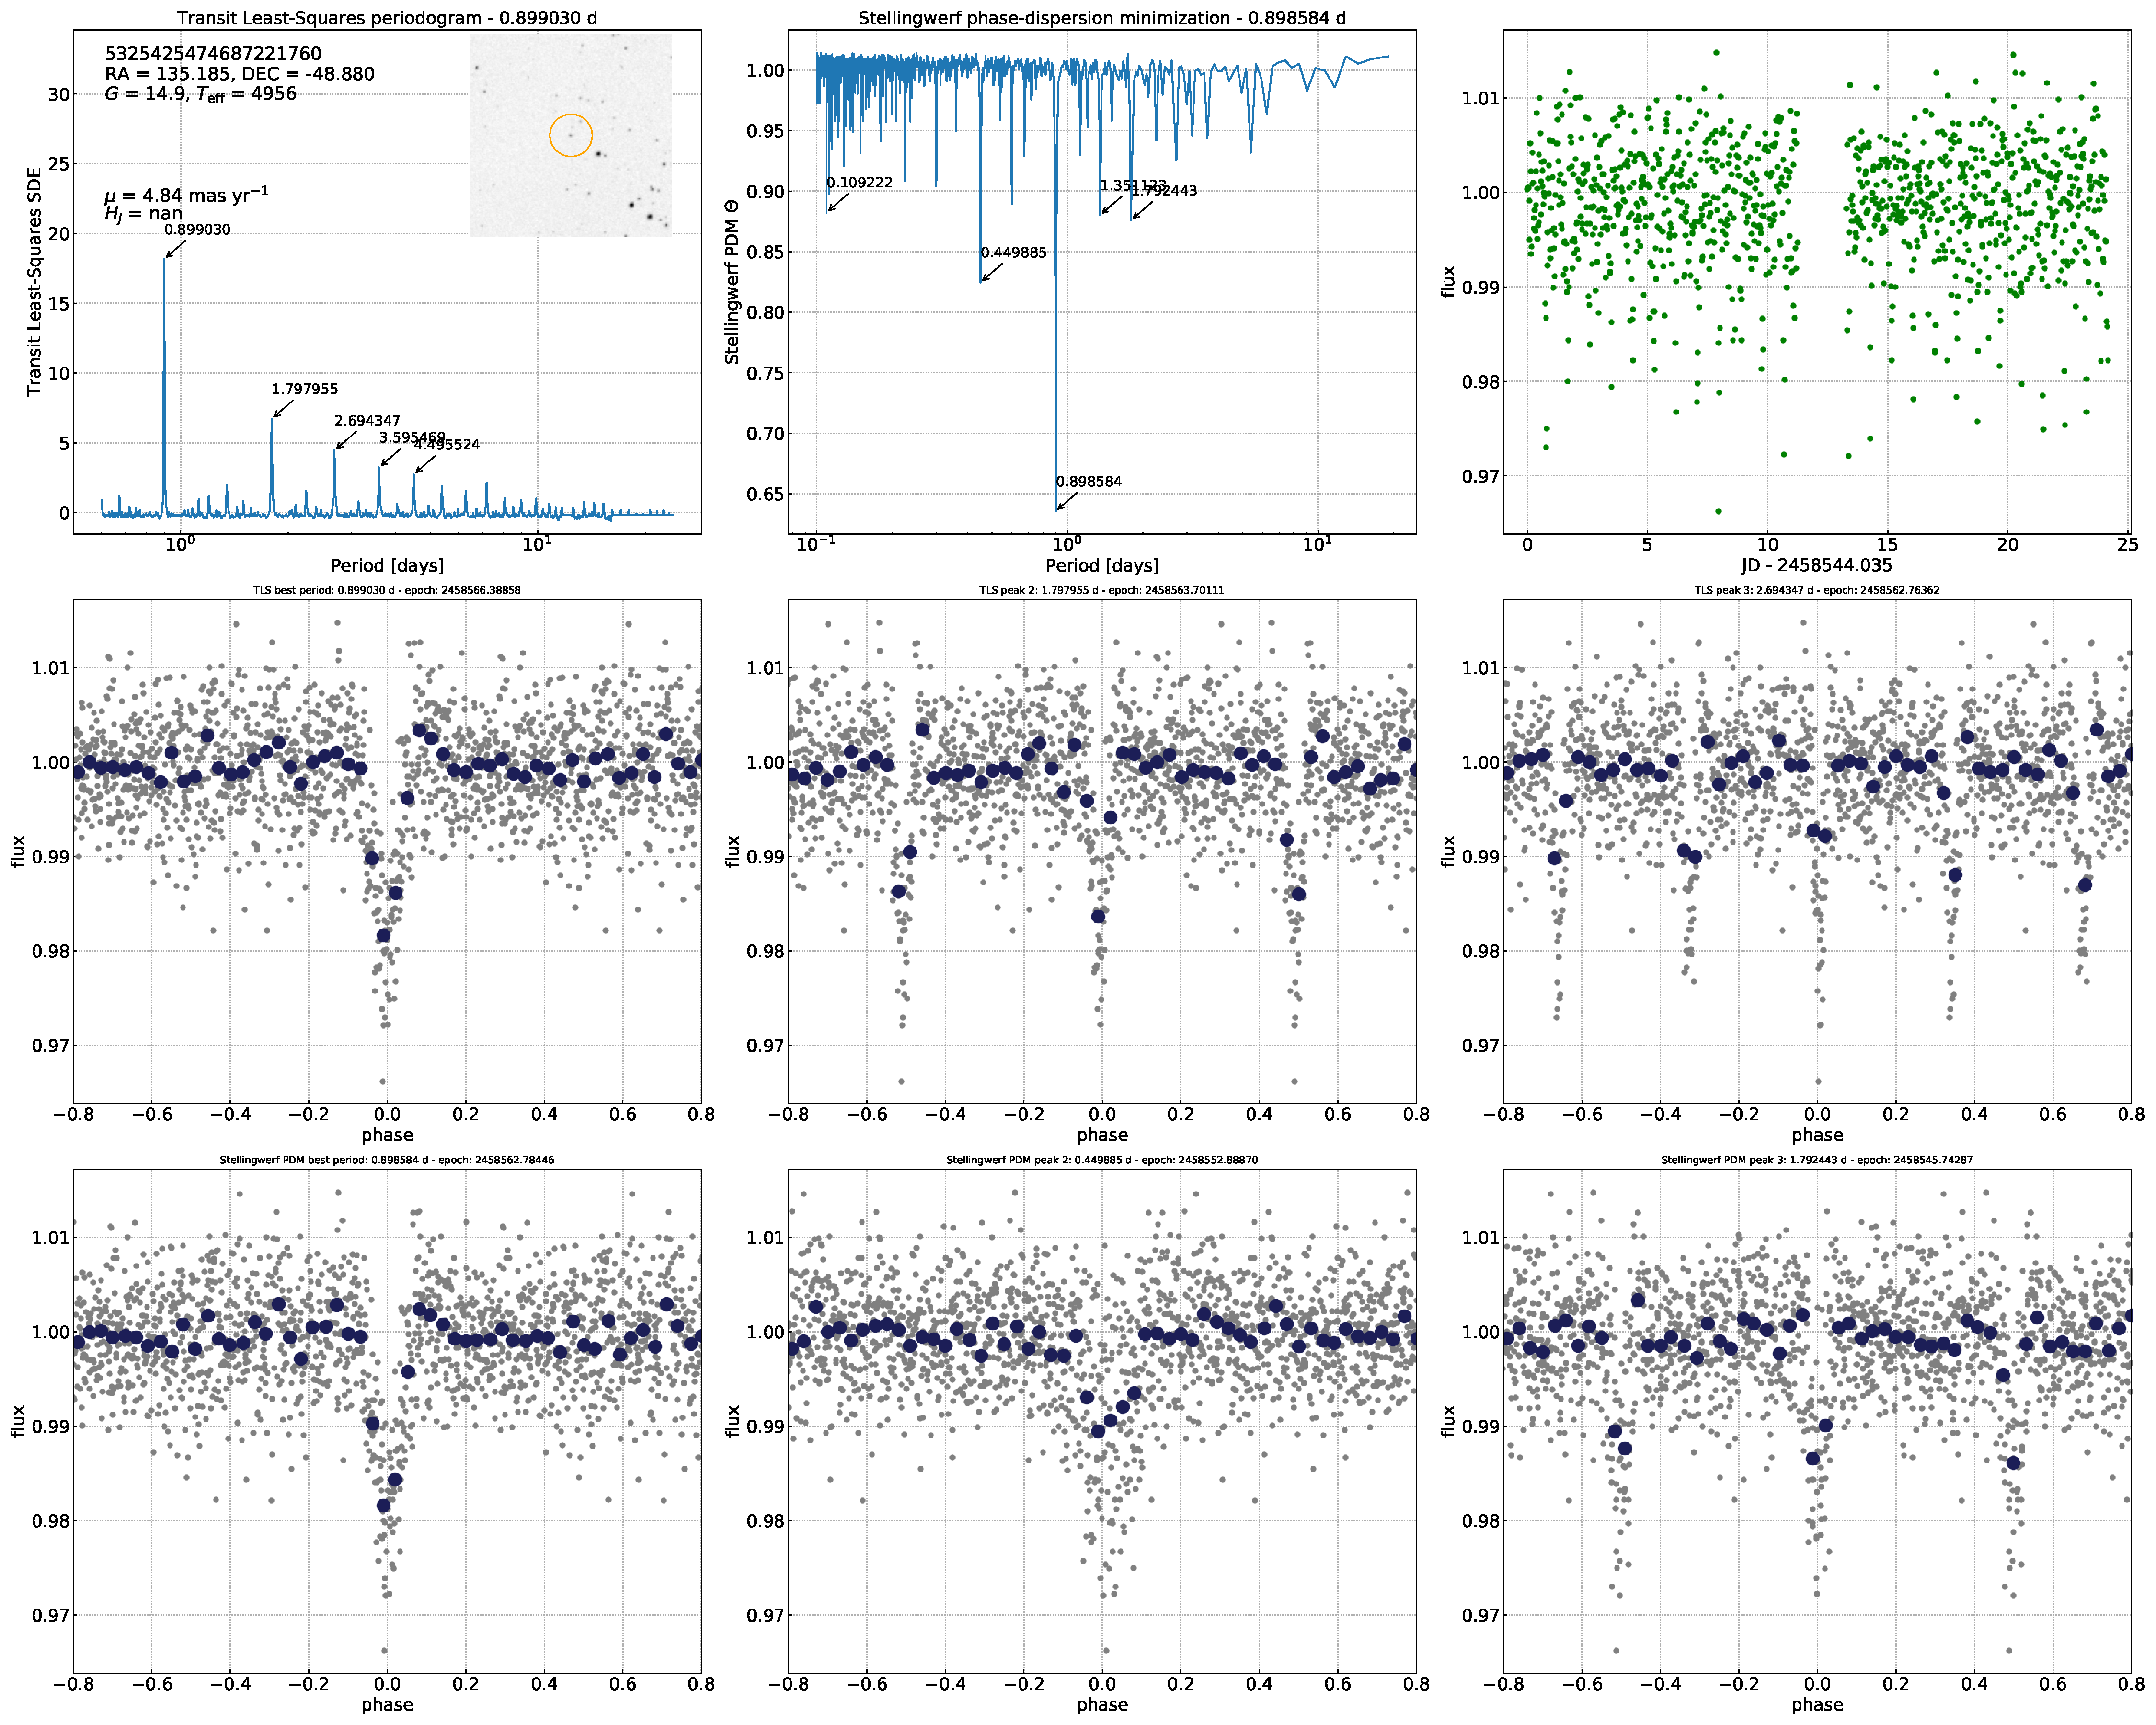
\includegraphics[width=0.8\textwidth]{pg_0001.pdf}
	\end{center}
	\vspace{-0.5cm}
	\caption{
    {\bf Transit search summary.} See \S~\ref{sec:pg1}.
		\label{fig:pg1}
	}
\end{figure*}

\begin{figure*}[!h]
	\begin{center}
		\leavevmode
		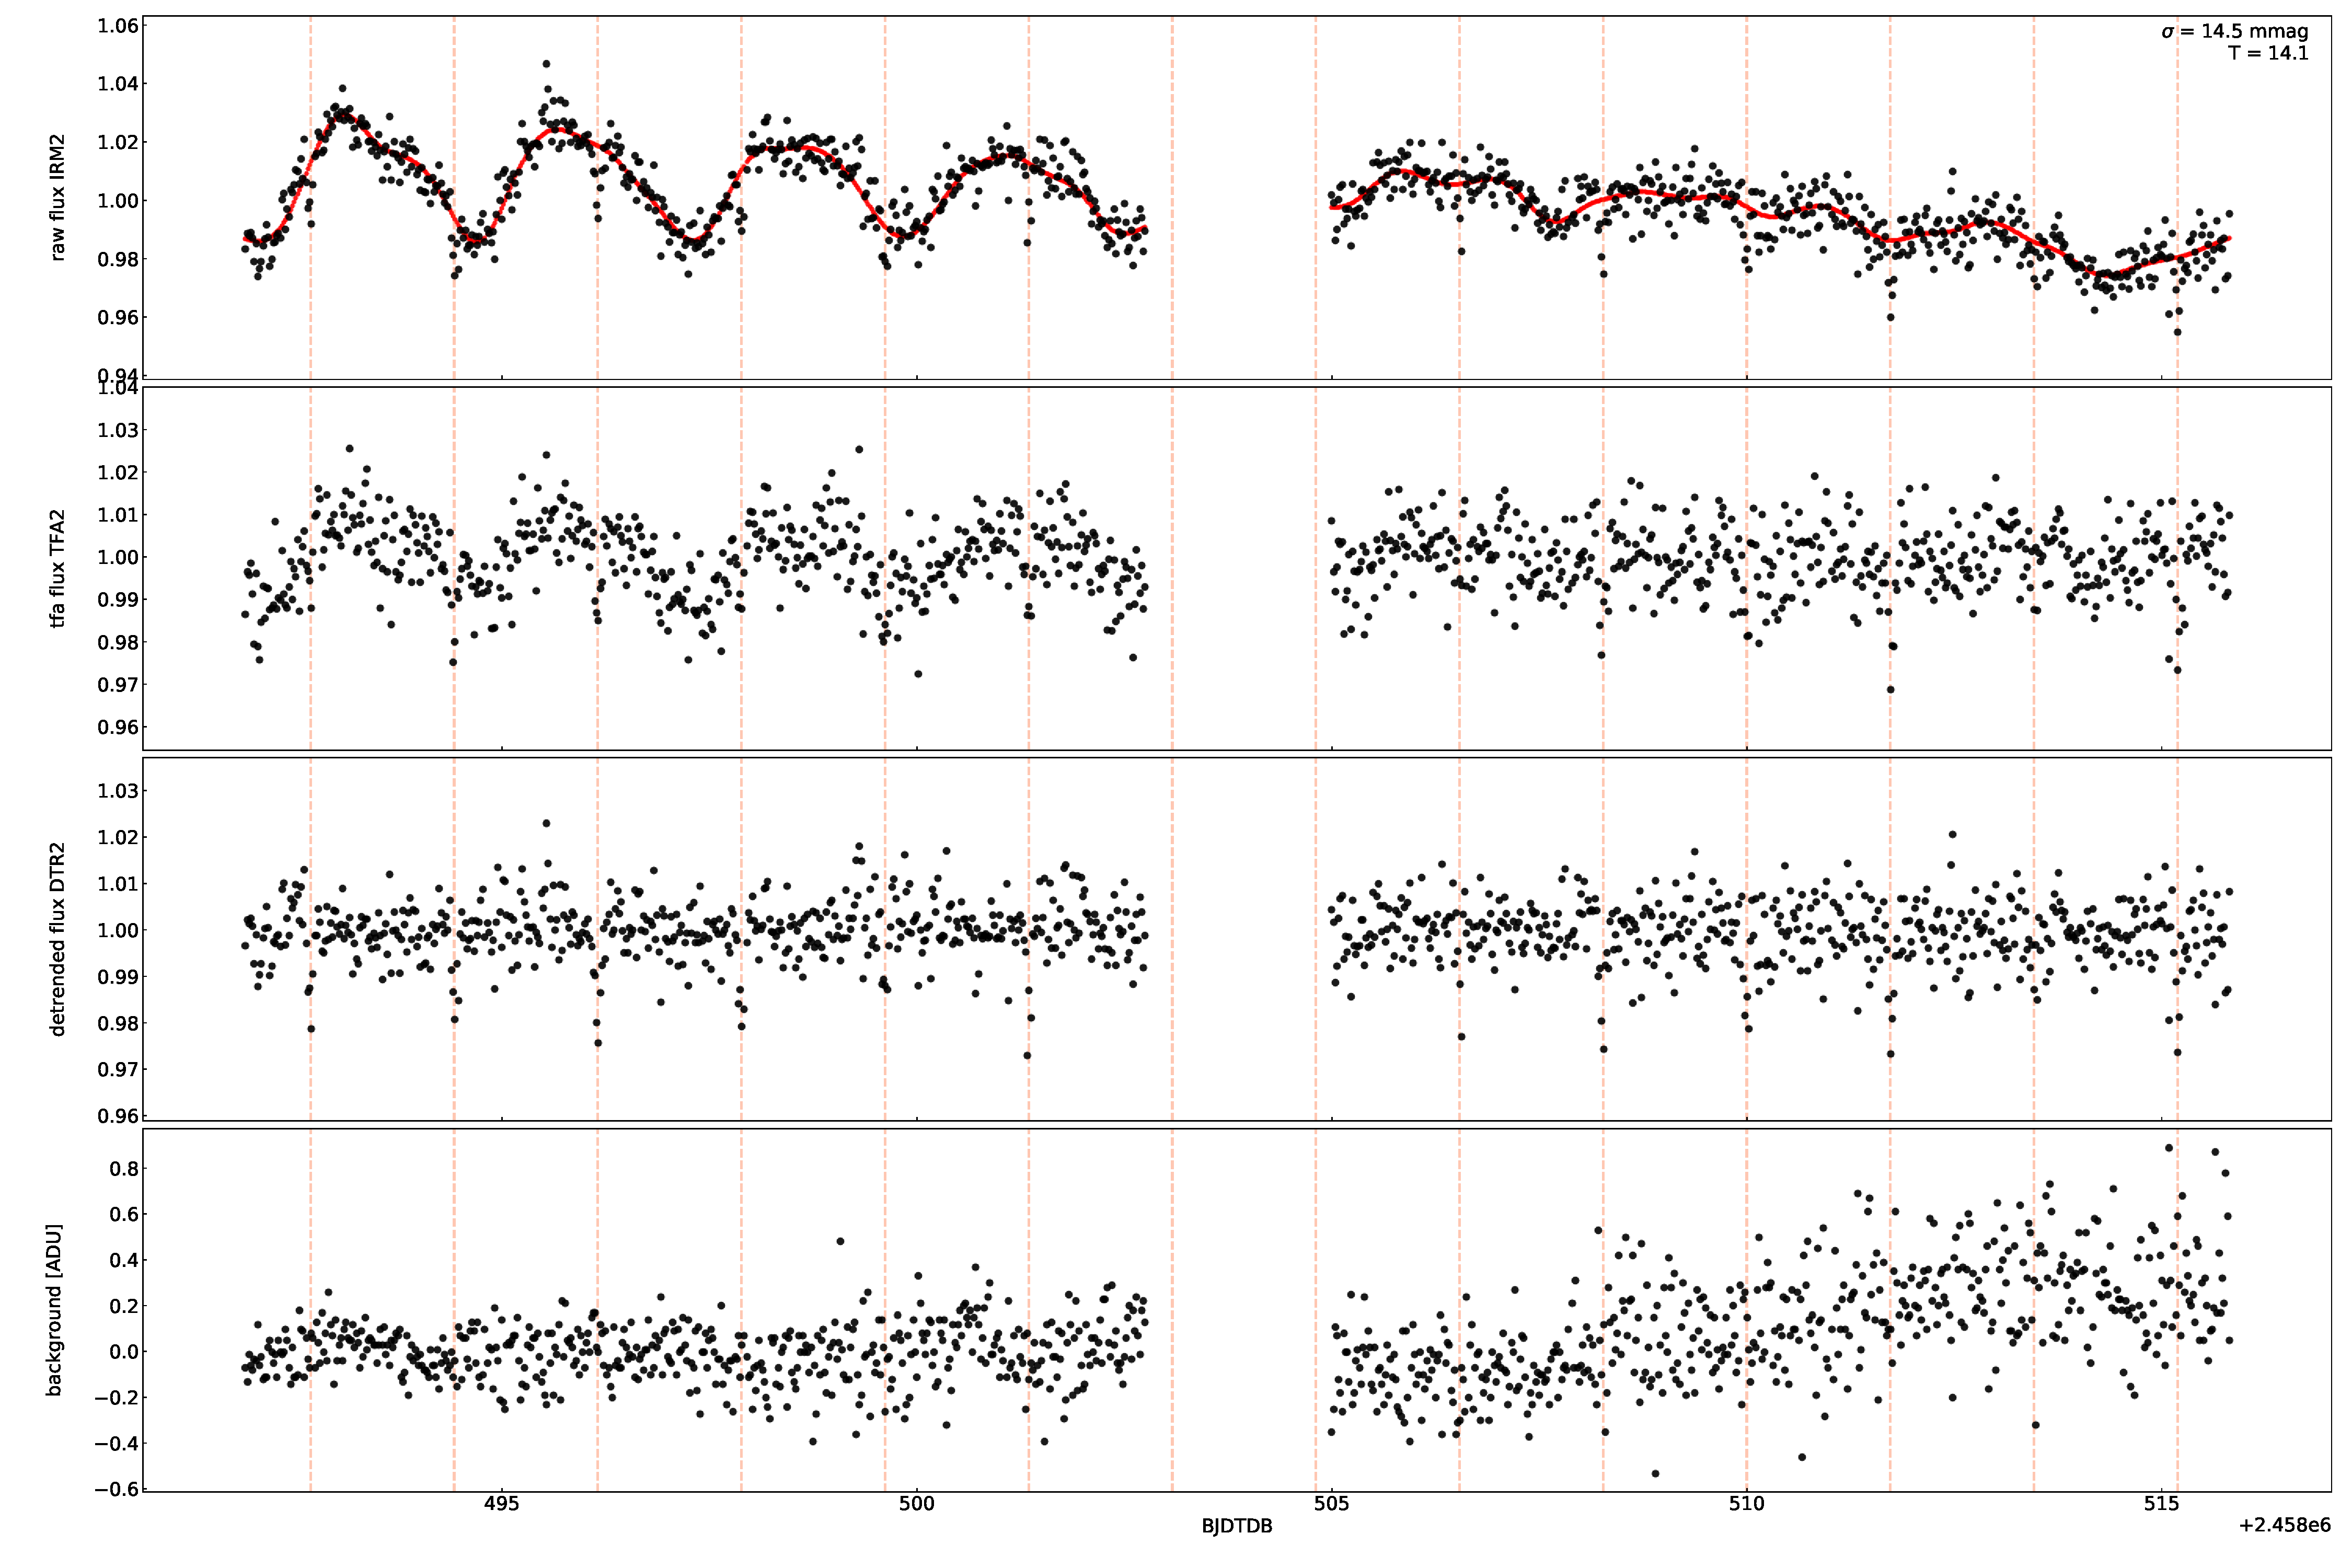
\includegraphics[width=0.8\textwidth]{pg_0002.pdf}
	\end{center}
	\vspace{-0.5cm}
	\caption{
		{\bf Light-curve diagnostics.} See \S~\ref{sec:pg2}.
		\label{fig:pg2}
	}
\end{figure*}

\begin{figure*}[!h]
	\begin{center}
		\leavevmode
		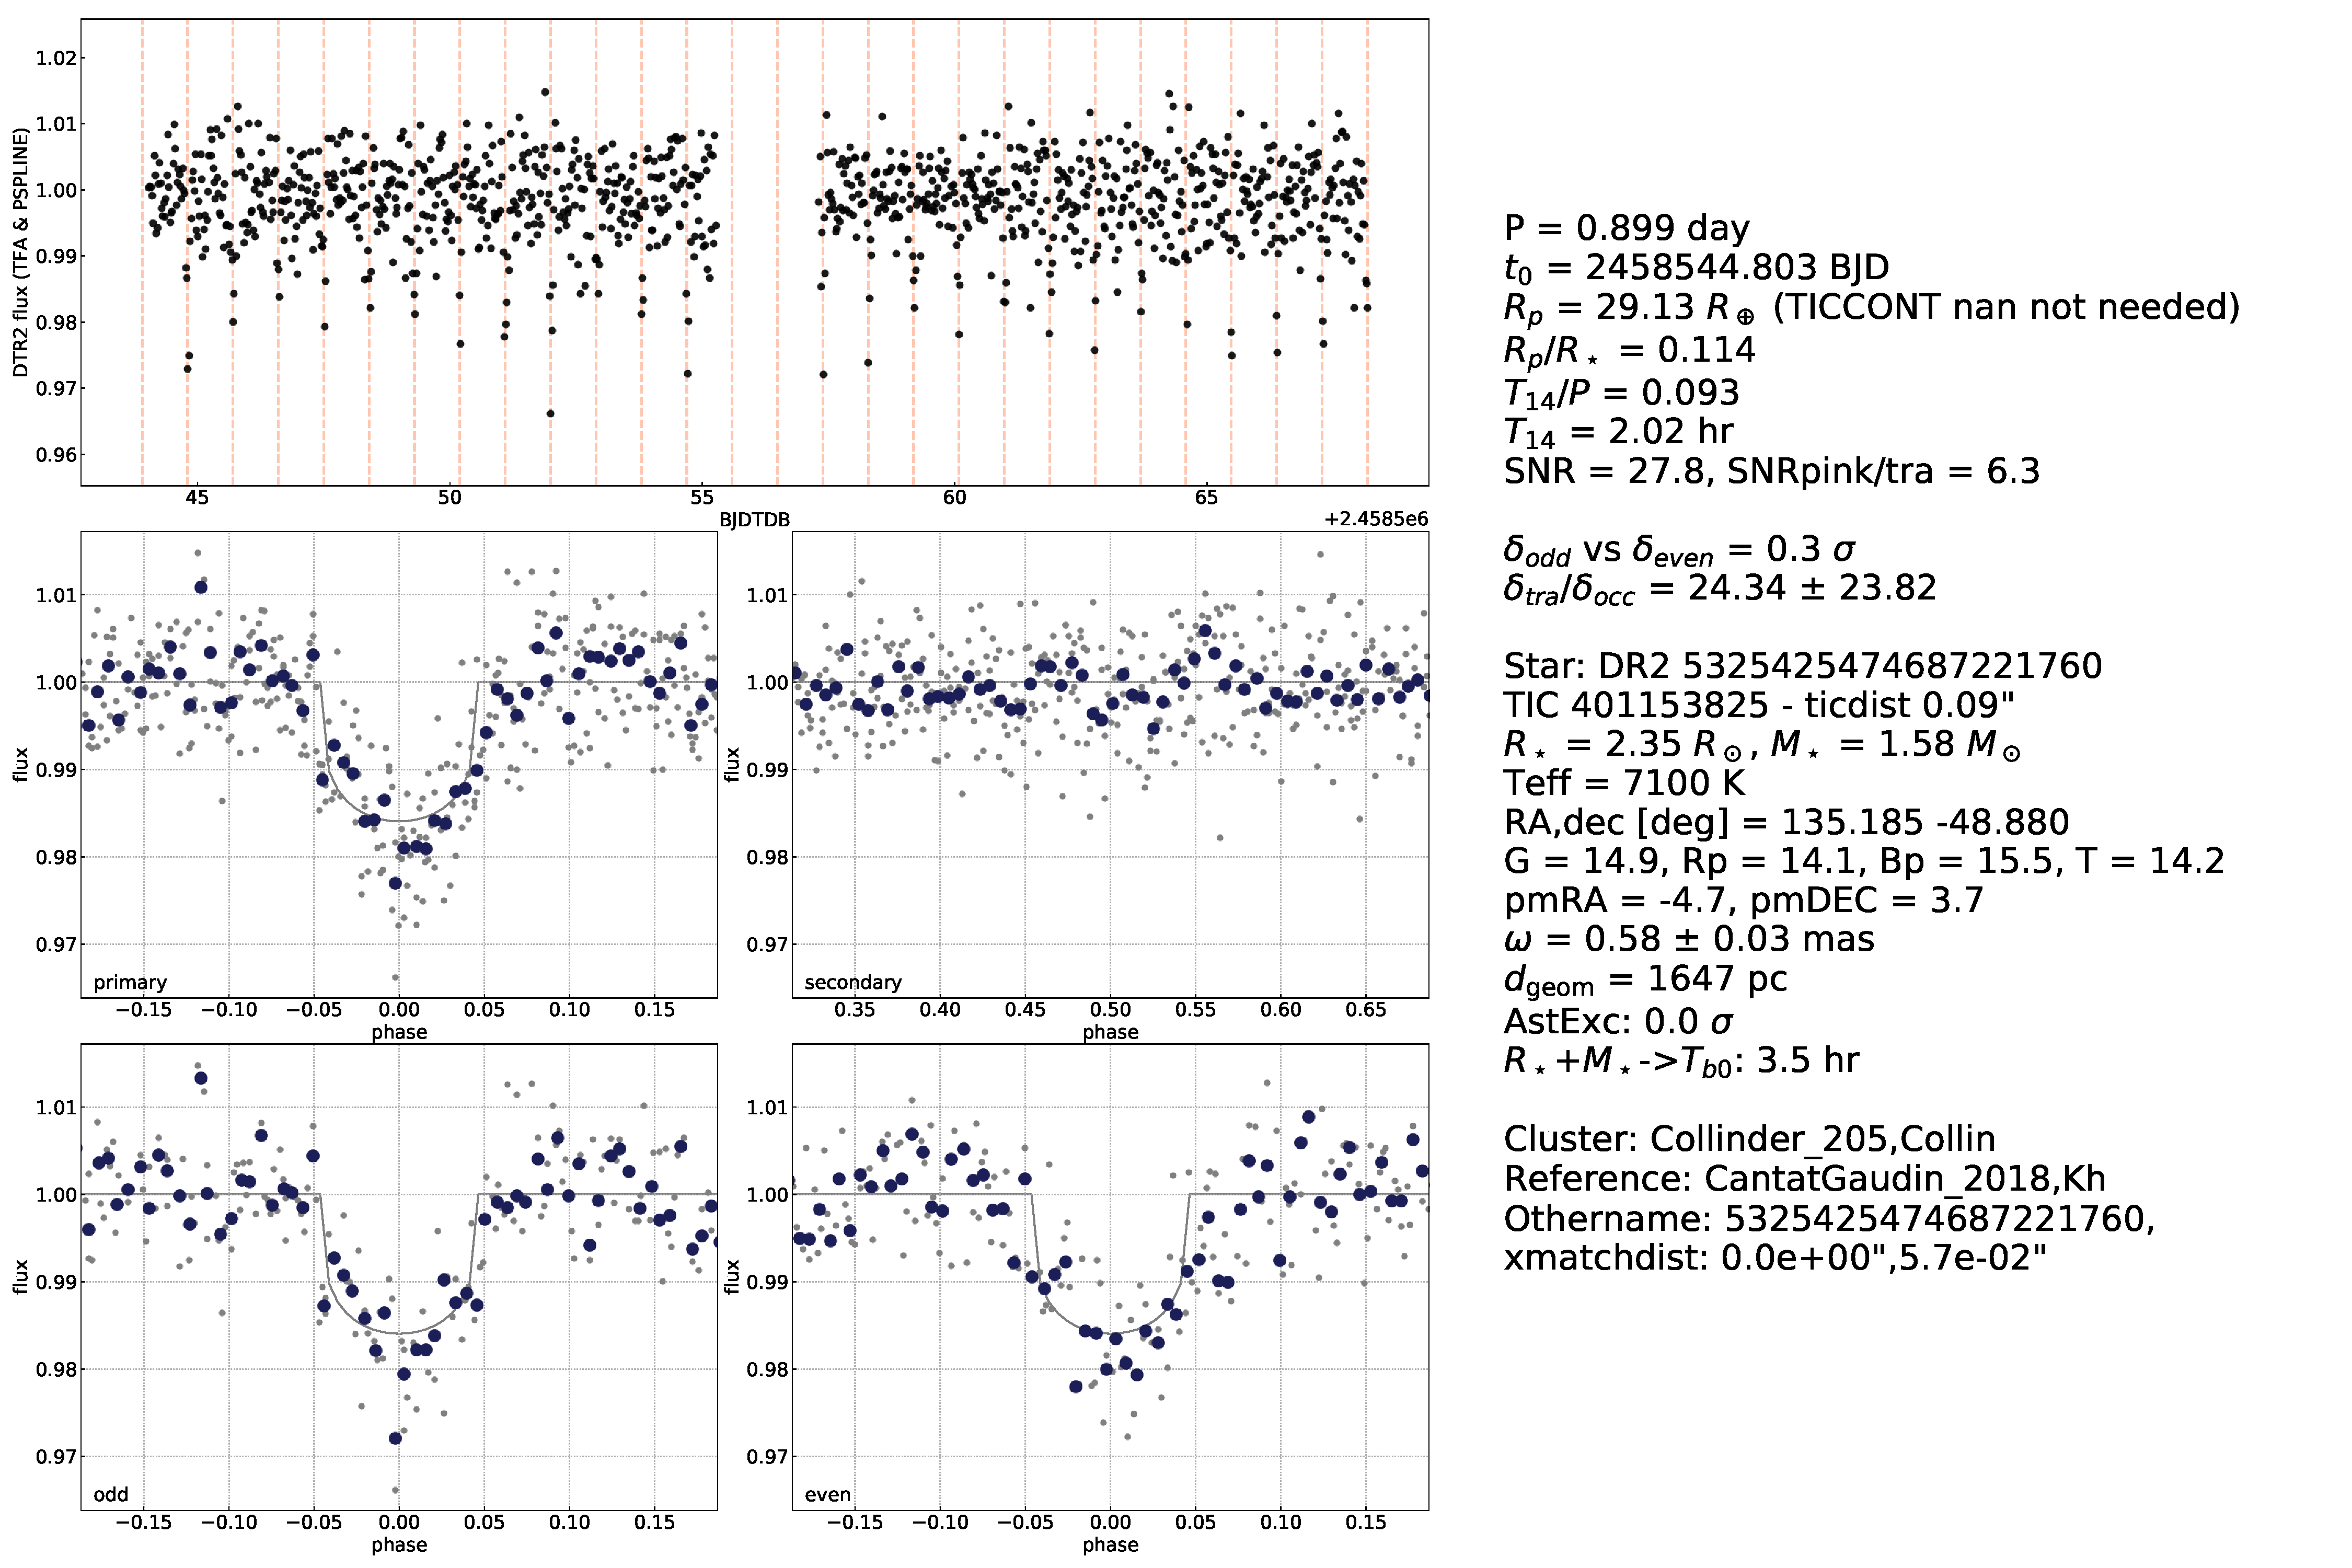
\includegraphics[width=0.8\textwidth]{pg_0003.pdf}
	\end{center}
	\vspace{-0.5cm}
	\caption{
    {\bf Transit diagnostics.}  See \S~\ref{sec:pg3}.
		\label{fig:pg3}
	}
\end{figure*}

\begin{figure*}[!h]
	\begin{center}
		\leavevmode
		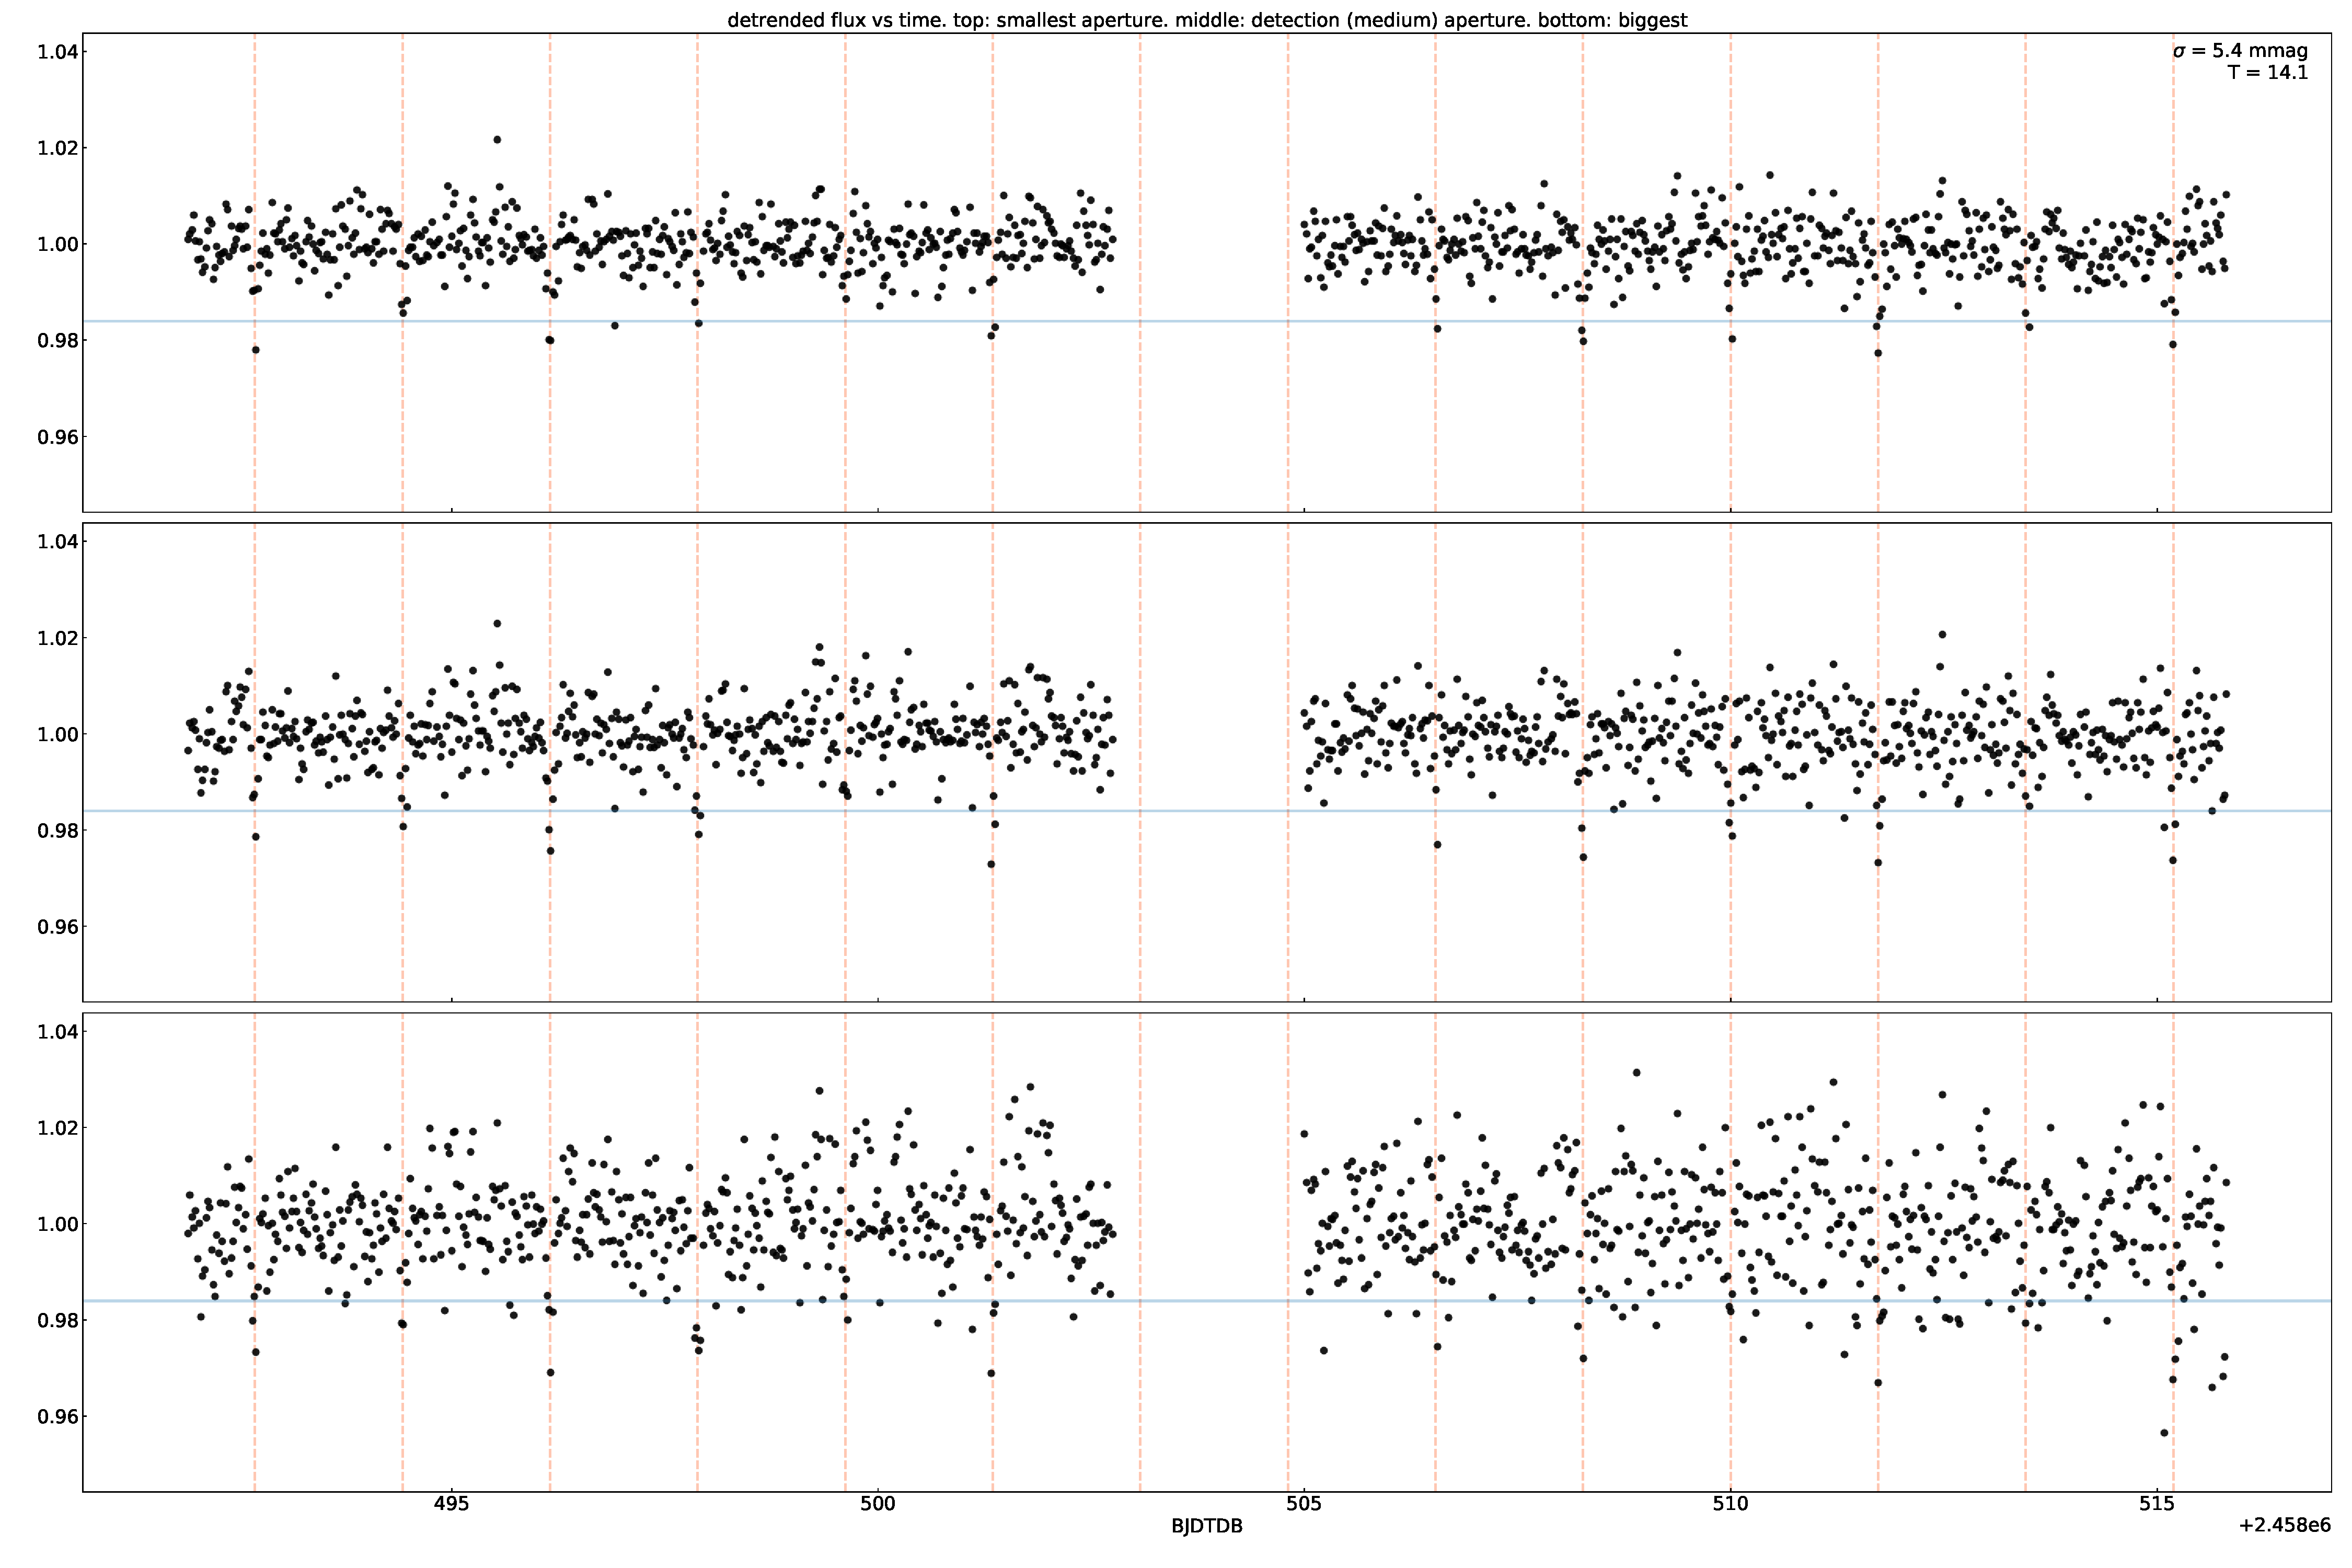
\includegraphics[width=0.8\textwidth]{pg_0004.pdf}
	\end{center}
	\vspace{-0.5cm}
	\caption{
		{\bf Light-curves for increasing aperture sizes.}  See
    \S~\ref{sec:pg4}.
		\label{fig:pg4}
	}
\end{figure*}

\begin{figure*}[!h]
	\begin{center}
		\leavevmode
		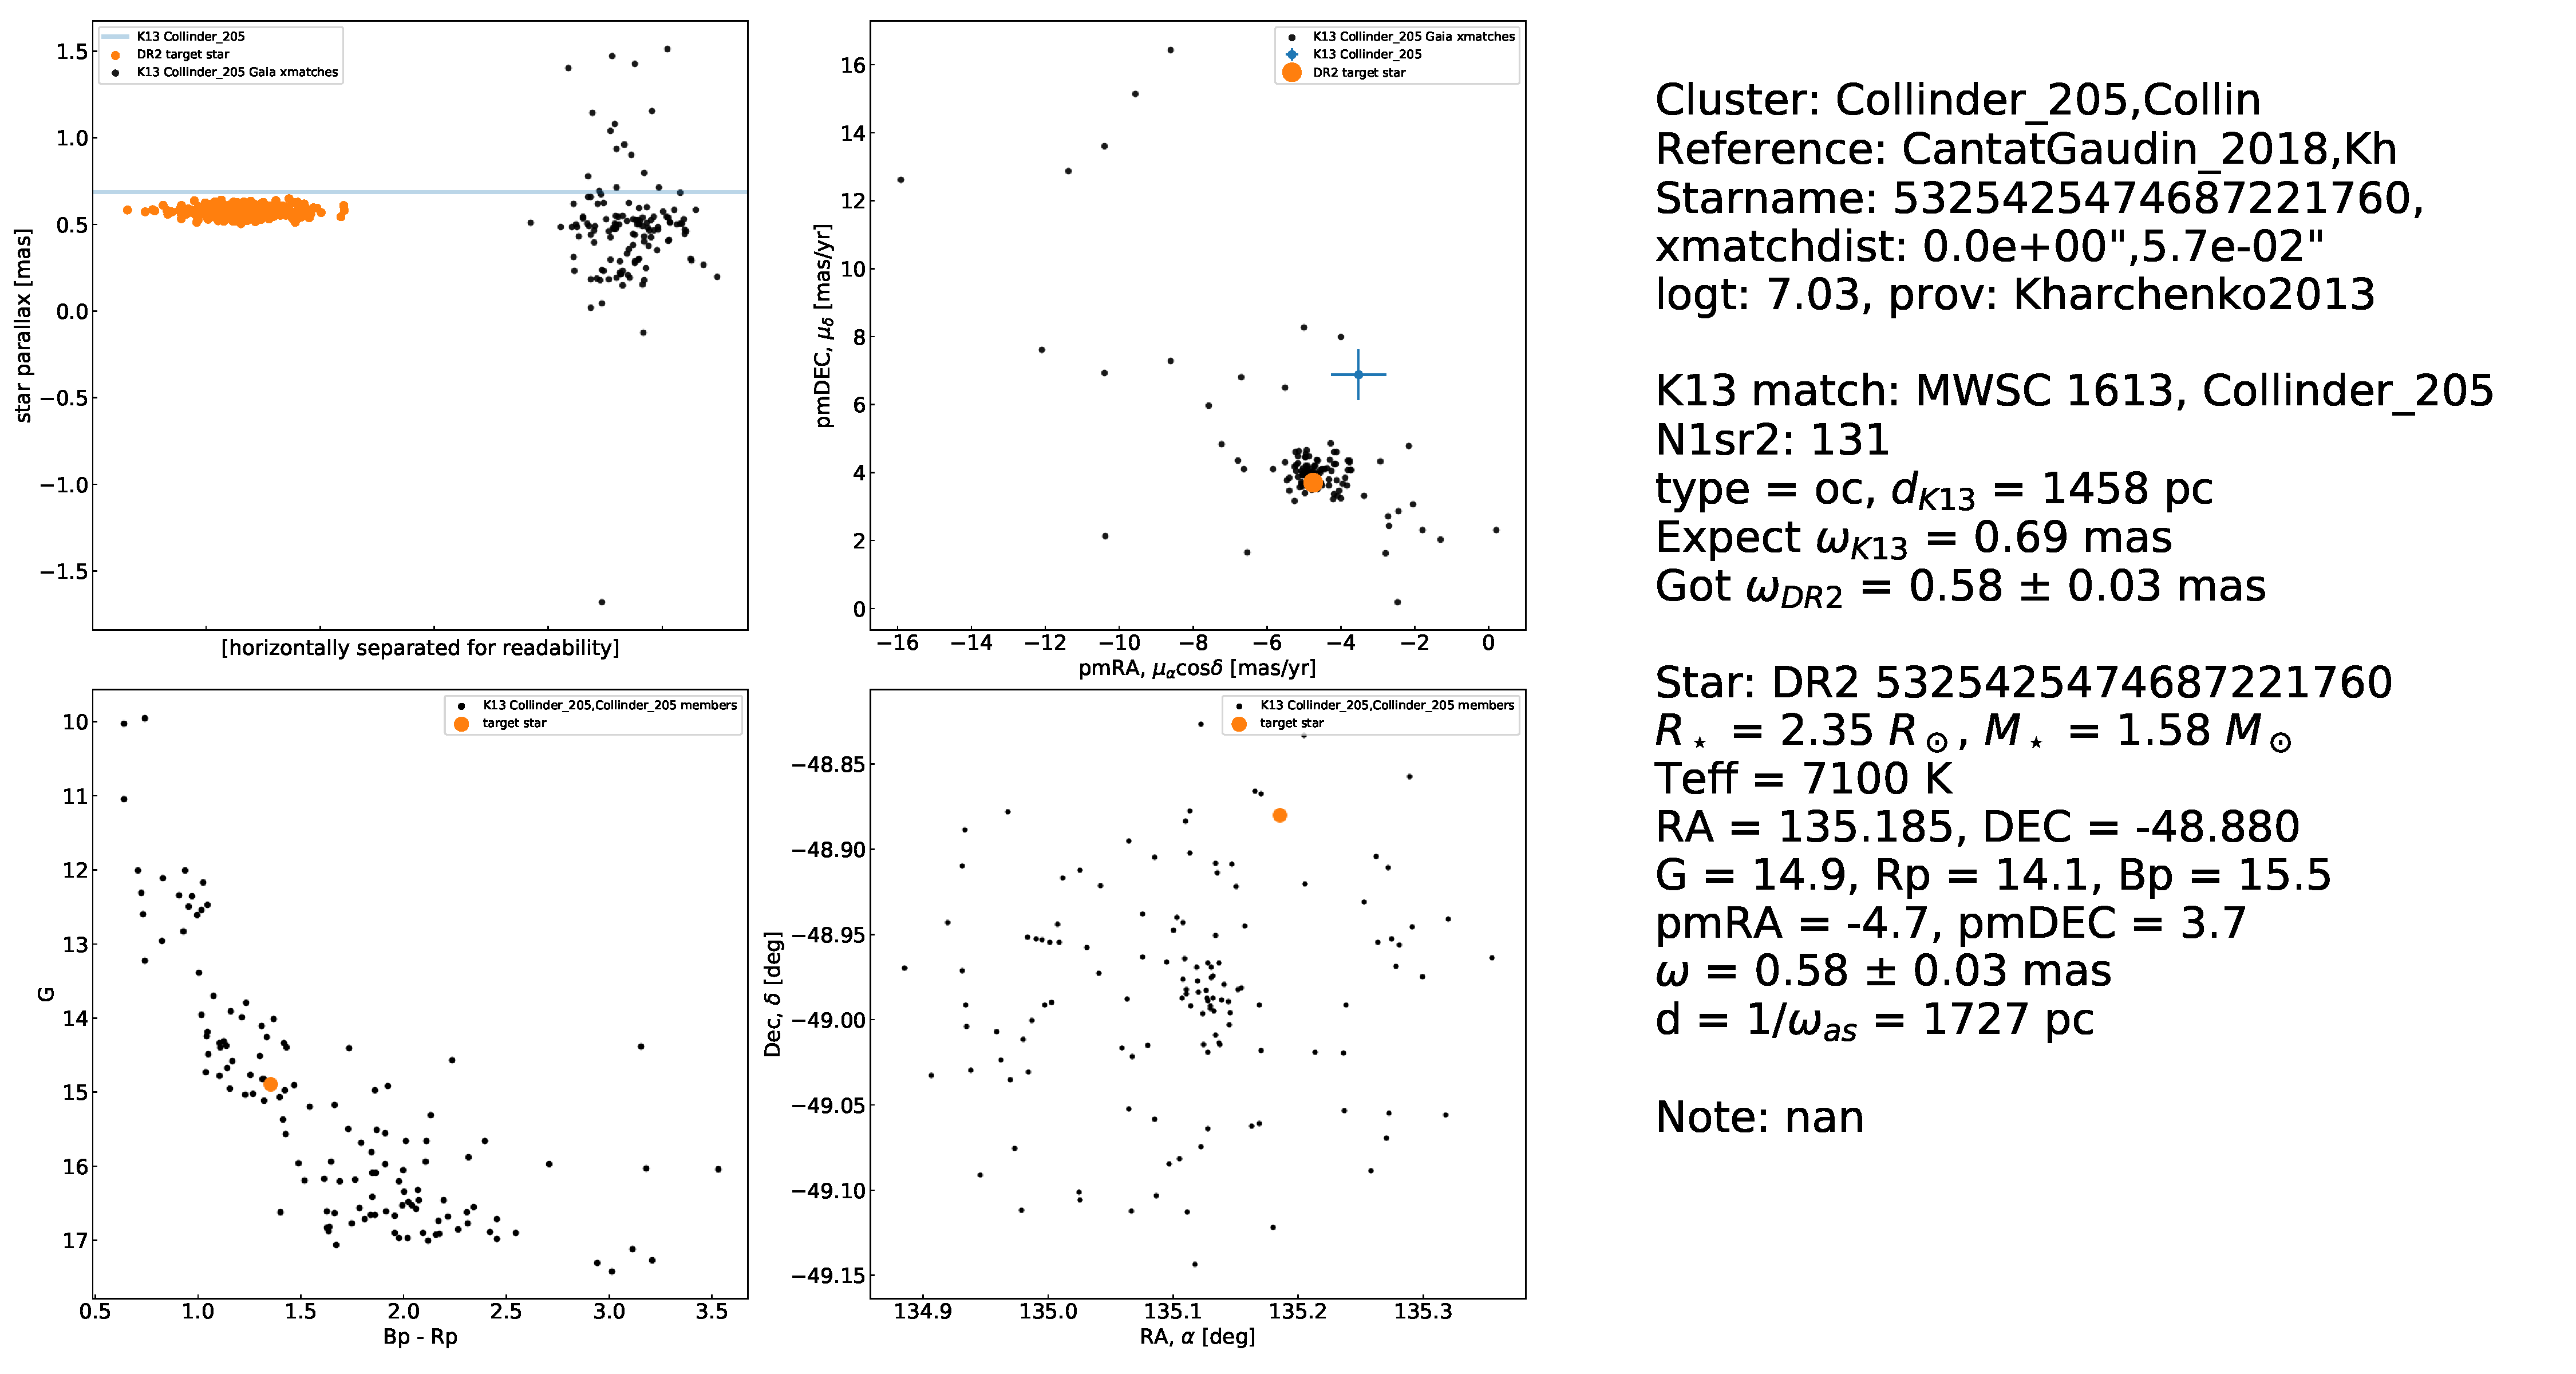
\includegraphics[width=0.8\textwidth]{pg_0005.pdf}
	\end{center}
	\vspace{-0.5cm}
	\caption{
    {\bf Cluster membership assessment diagnostics.} See
    \S~\ref{sec:pg5}.
		\label{fig:pg5}
	}
\end{figure*}

\begin{figure*}[!h]
	\begin{center}
		\leavevmode
		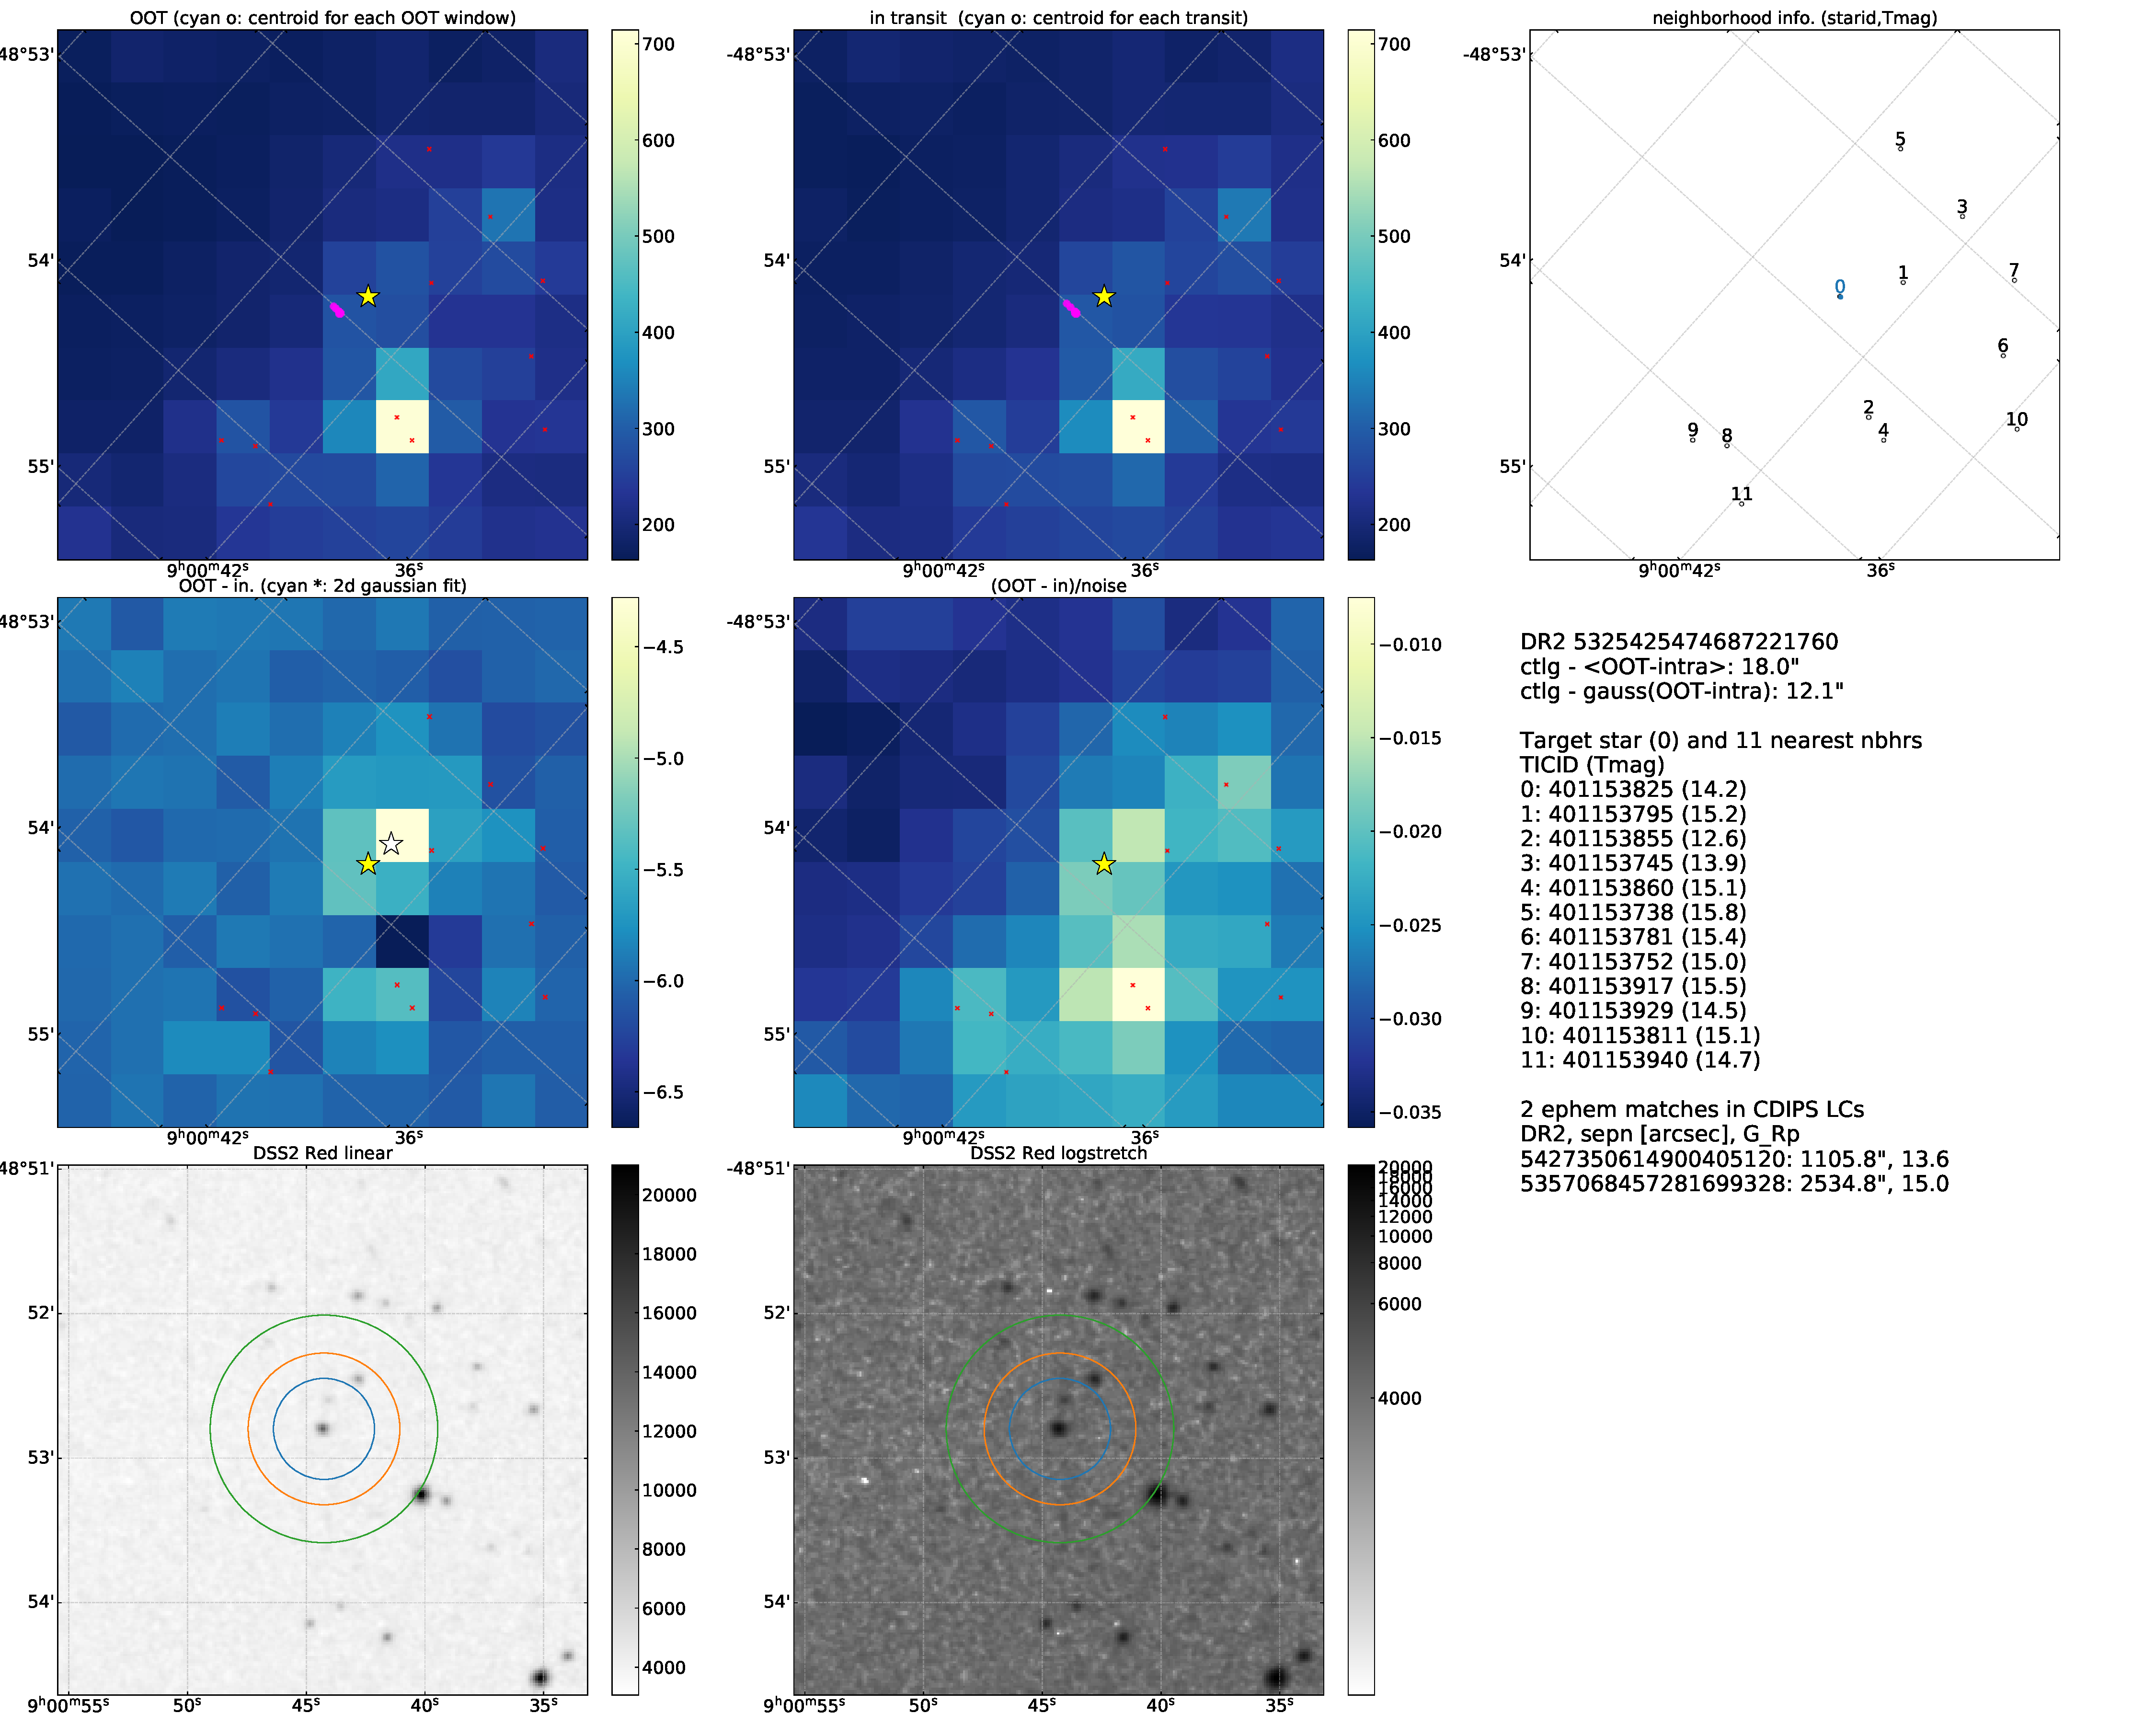
\includegraphics[width=0.8\textwidth]{pg_0006.pdf}
	\end{center}
	\vspace{-0.5cm}
	\caption{
		{\bf Imaging variability diagnostics.} See \S~\ref{sec:pg6}.
		\label{fig:pg6}
	}
\end{figure*}

\begin{figure*}[!h]
	\begin{center}
		\leavevmode
		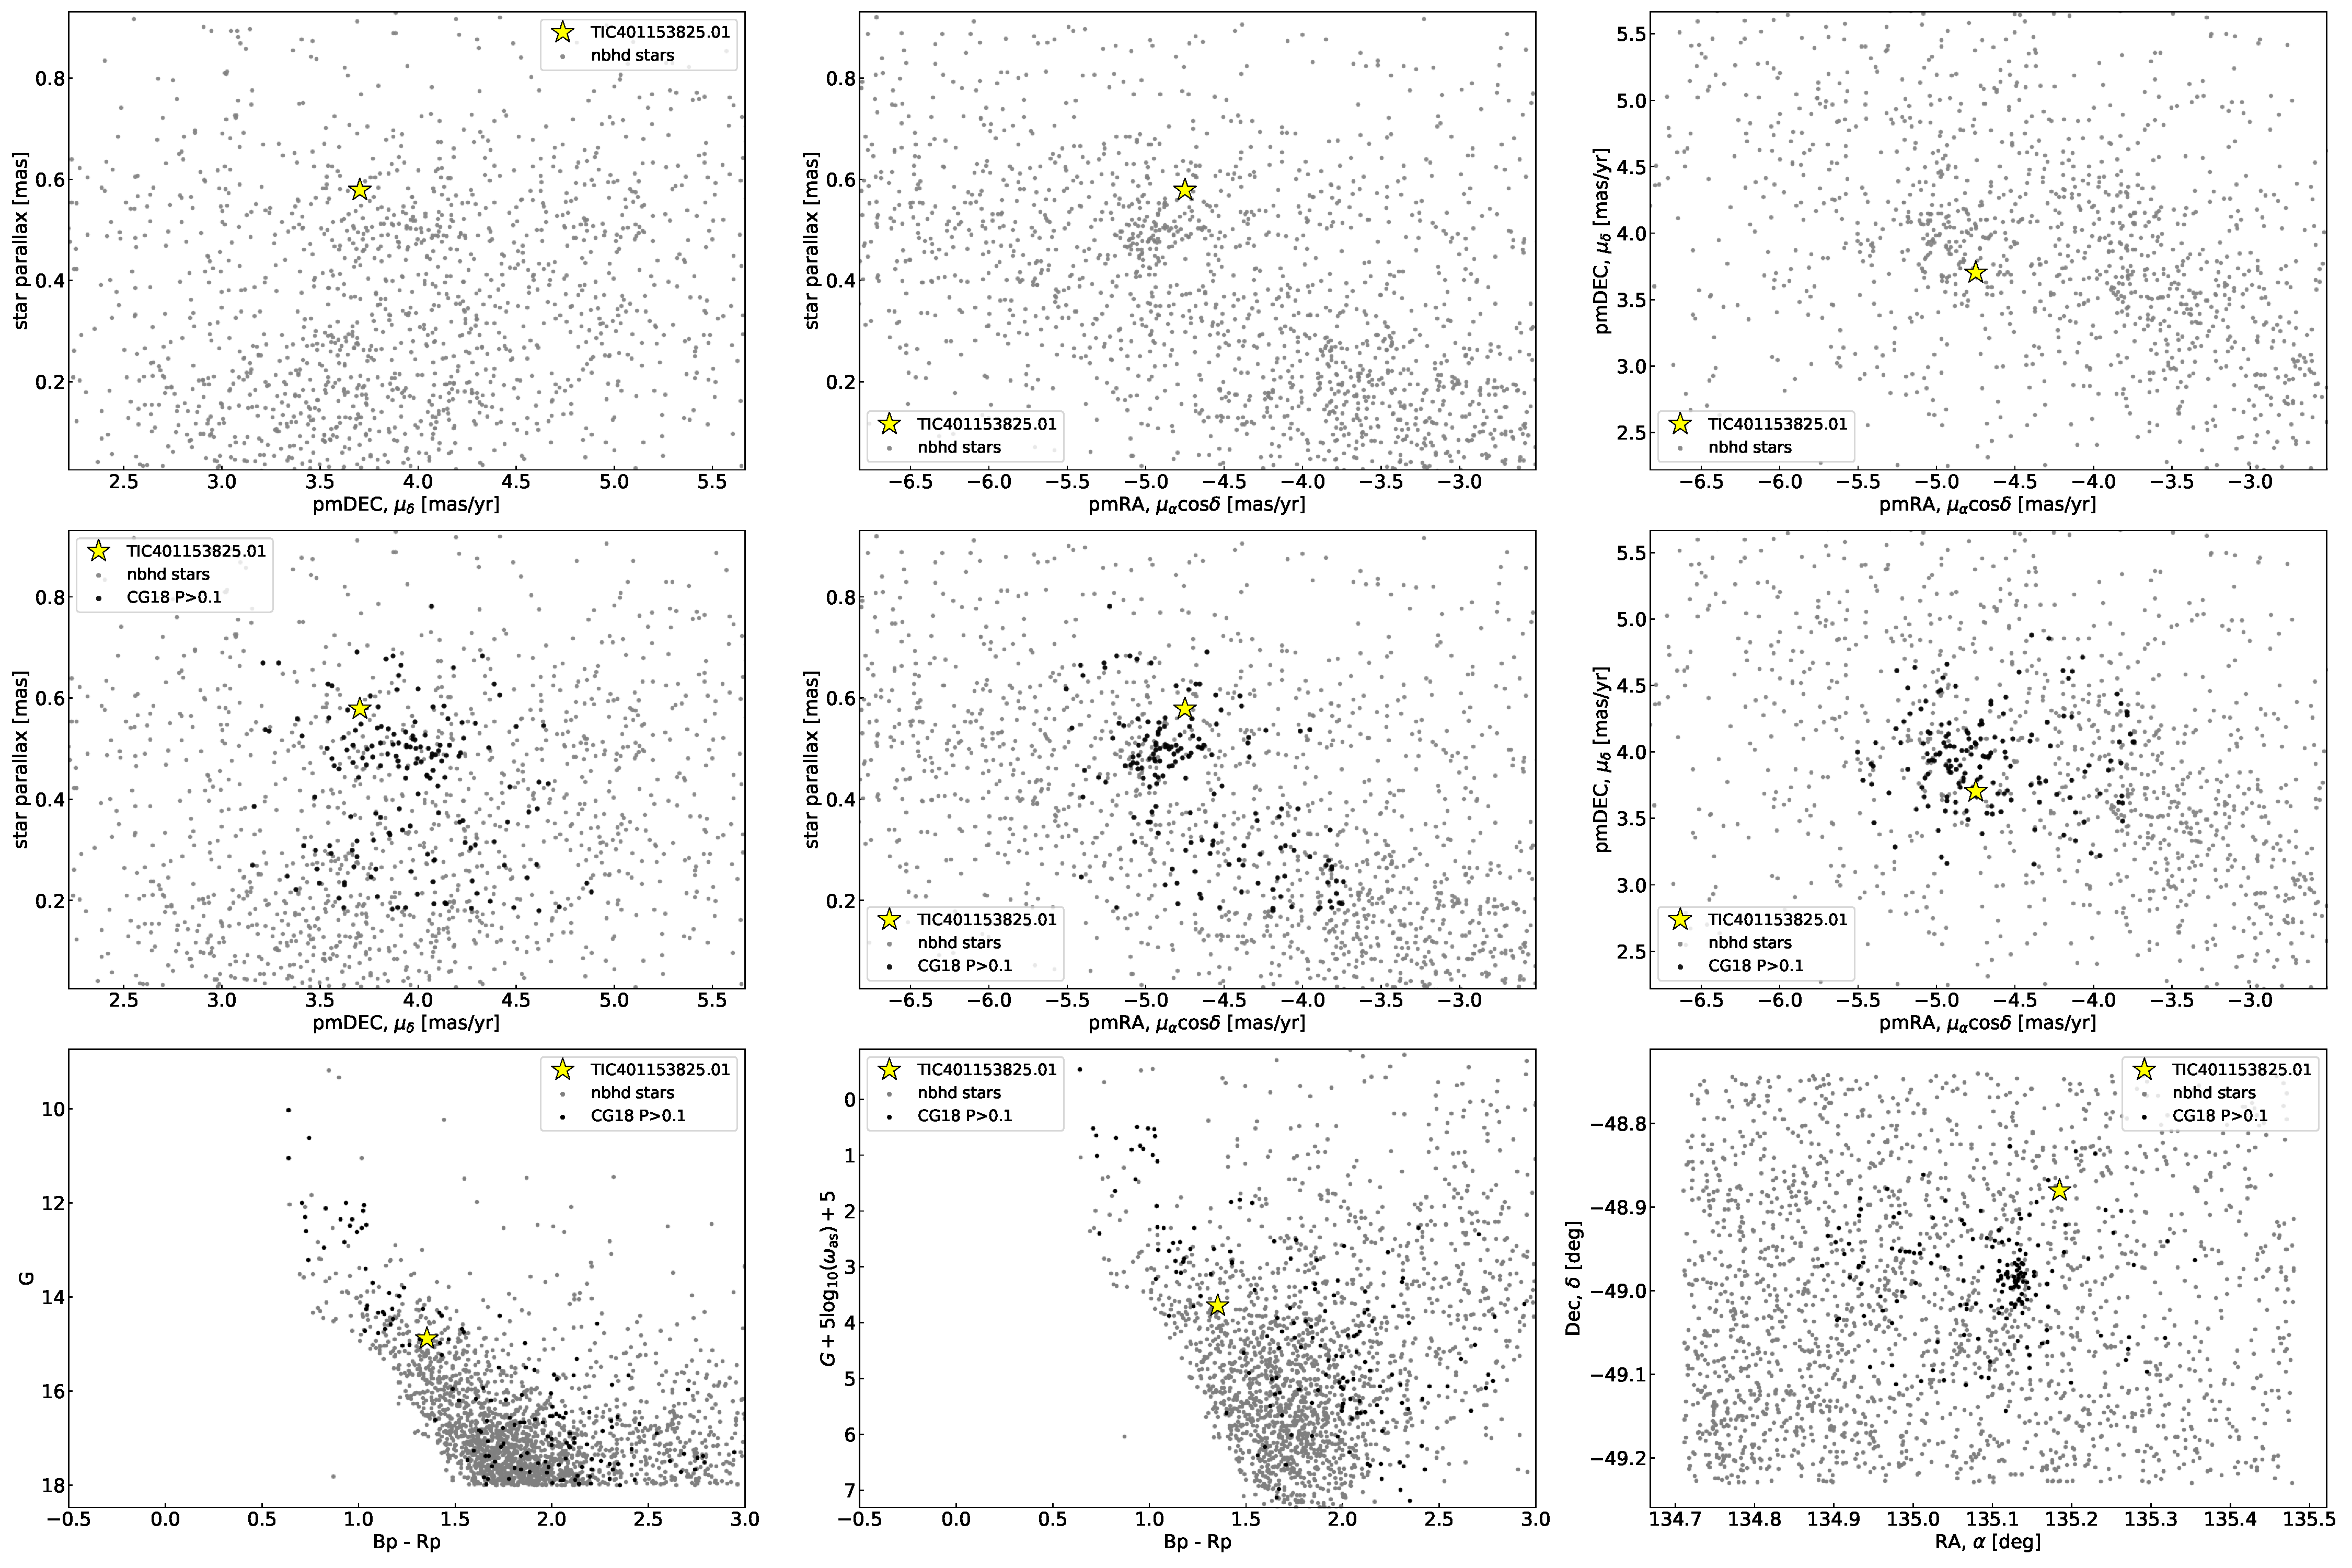
\includegraphics[width=0.85\textwidth]{pg_0007.pdf}
	\end{center}
	\vspace{-0.5cm}
	\caption{
		{\bf Neighborhood diagnostic.} See \S~\ref{sec:pg7}.
		\label{fig:pg7}
	}
\end{figure*}


%%%%%%%%%%%
% BIBLIOGRAPHY %
%%%%%%%%%%%
\clearpage
\newpage
\bibliographystyle{yahapj}                            
\bibliography{bibliography} 

\end{document}

